%!TEX root = ../slides.tex
\section{Future work}
\begin{frame}{Future work}{Pending tasks}
\begin{table}
%\renewcommand{\arraystretch}{1.2}
\centering
\resizebox{0.9\textwidth}{!}{%
\begin{tabular}{lllllllllllllll}
   &                                                                                                                             & \multicolumn{5}{c}{2017}                                                                                                                  & \multicolumn{8}{c}{2018}                                                                                                                                                                                                      \\
   \toprule
\# & \multicolumn{1}{c}{Activity}                                                                                                & \multicolumn{1}{c}{\scriptsize{Aug}}   & \multicolumn{1}{c}{\scriptsize{Sep}}   & \multicolumn{1}{c}{\scriptsize{Oct}}   & \multicolumn{1}{c}{\scriptsize{Nov}}   & \multicolumn{1}{c}{\scriptsize{Dec}}   & \multicolumn{1}{c}{\scriptsize{Jan}}   & \multicolumn{1}{c}{\scriptsize{Feb}}   & \multicolumn{1}{c}{\scriptsize{Mar}}   & \multicolumn{1}{c}{\scriptsize{Apr}}   & \multicolumn{1}{c}{\scriptsize{May}}   & \multicolumn{1}{c}{\scriptsize{Jun}}   & \multicolumn{1}{c}{\scriptsize{Jul}}   & \multicolumn{1}{c}{\scriptsize{Aug}}   \\
\midrule
\multicolumn{2}{c}{\textbf{Solution refinement activities}}                                                                               &                           &                           &                           &                           &                           &                           &                           &                           &                           &                           &                           &                           &                           \\
%\cmidrule{1-15}
1  & Incorporation of the HAR module in the CC                                                                                   & \cellcolor[HTML]{00D2CB} & \cellcolor[HTML]{00D2CB} &                           &                           &                           &                           &                           &                           &                           &                           &                           &                           &                           \\
\cmidrule[0.25pt]{1-15}
2  & \begin{tabular}[c]{@{}l@{}}Incorporation of the accuracy requirement in\\ the CC\end{tabular}                               &                           & \cellcolor[HTML]{00D2CB} & \cellcolor[HTML]{00D2CB} &                           &                           &                           &                           &                           &                           &                           &                           &                           &                           \\ 
\cmidrule[0.75pt]{1-15}
\multicolumn{2}{c}{\rule{0pt}{4ex}\textbf{On-device implementation}}                                                                &                           &                           &                           &                           &                           &                           &                           &                           &                           &                           &                           &                           &                           \\
%\cmidrule{1-15}
3  & \rule{0pt}{2ex}Implementation of sigmoid-driven sampling                                                                                     &                           &                           &                           & \cellcolor[HTML]{00D2CB} &                           &                           &                           &                           &                           &                           &                           &                           &                           \\
\cmidrule[0.25pt]{1-15}
4  & \begin{tabular}[c]{@{}l@{}}Watchdog mechanisms for \emph{Geofencing} and\\ \emph{Sampling Decision Maker} modules\end{tabular}            &                           &                           &                           & \cellcolor[HTML]{00D2CB} &                           &                           &                           &                           &                           &                           &                           &                           &                           \\
\cmidrule[0.25pt]{1-15}
5  & \begin{tabular}[c]{@{}l@{}}Refinement of the list of candidate stay points\\ employed by the \emph{Geofencing} module\end{tabular} &                           &                           &                           & \cellcolor[HTML]{00D2CB} & \cellcolor[HTML]{00D2CB} &                           &                           &                           &                           &                           &                           &                           &                           \\
\cmidrule[0.5pt]{1-15}


\multicolumn{2}{c}{\rule{0pt}{4ex}\textbf{Experimentation}}                                                                &                           &                           &                           &                           &                           &                           &                           &                           &                           &                           &                           &                           &                           \\
6  & \begin{tabular}[c]{@{}l@{}}Experiments with larger\\and heterogeneous mobility\end{tabular}                     &                           &                           &                           &                           &                           & \cellcolor[HTML]{00D2CB} & \cellcolor[HTML]{00D2CB} & \cellcolor[HTML]{00D2CB} &                           &                           &                           &                           &                           \\
\cmidrule[0.25pt]{1-15}
7  & Completion of evaluation framework                                                                                          &                           &                           &                           &                           & \cellcolor[HTML]{00D2CB} & \cellcolor[HTML]{00D2CB} & \cellcolor[HTML]{00D2CB} &                           &                           &                           &                           &                           &                           \\
\cmidrule[0.25pt]{1-15}
8  & Comparison with other solutions                                                                                             &                           &                           &                           &                           &                           &                           &                           &                           & \cellcolor[HTML]{00D2CB} & \cellcolor[HTML]{00D2CB} &                           &                           &                           \\
\cmidrule[0.5pt]{1-15}


\multicolumn{2}{c}{\rule{0pt}{4ex}\textbf{Research work activities}}                                                                                     &                           &                           &                           &                           &                           &                           &                           &                           &                           &                           &                           &                           &                           \\
%\cmidrule{1-15}
9  & \rule{0pt}{2ex}Thesis writing-review                                                                                                       &                           &                           &                           &                           &                           &                           &                           & \cellcolor[HTML]{00D2CB} & \cellcolor[HTML]{00D2CB} & \cellcolor[HTML]{00D2CB} & \cellcolor[HTML]{00D2CB} & \cellcolor[HTML]{00D2CB} &                           \\
\cmidrule[0.25pt]{1-15}
10 & Thesis defense                                                                                                              &                           &                           &                           &                           &                           &                           &                           &                           &                           &                           &                           &                           & \cellcolor[HTML]{00D2CB} \\
\bottomrule
\end{tabular}
}
\caption{Schedule of pending activities of the research work for the last year of the doctoral program.}
\label{tab:schedule}
\end{table}
\end{frame}

\begin{frame}{Future work}{Incorporation of the HAR module in the CC}
\small
\vspace{-0.3cm}
\begin{block}{\small \textbf{Incorporation of the HAR module in the CC}}
\begin{itemize}
	\item For aiding the detection of departures in stay point mode:
	\begin{itemize}
		\item The center segments of the generated sigmoid sampling could employ HAR instead of GPS location updates. 
		GPS can confirm the motion detection.
		\item It could avoid the fixed \emph{conservative sampling} of the late departure mismatch reaction.
	\end{itemize}

	\item For adaptive GPS sampling during trajectory mode:
	\begin{itemize}
		\item A consecutive static outcome from the HAR module could reduce GPS sampling rate, otherwise it could be incremented according to detected transportation mode.
	\end{itemize}
\end{itemize}
\end{block}

\begin{figure}
  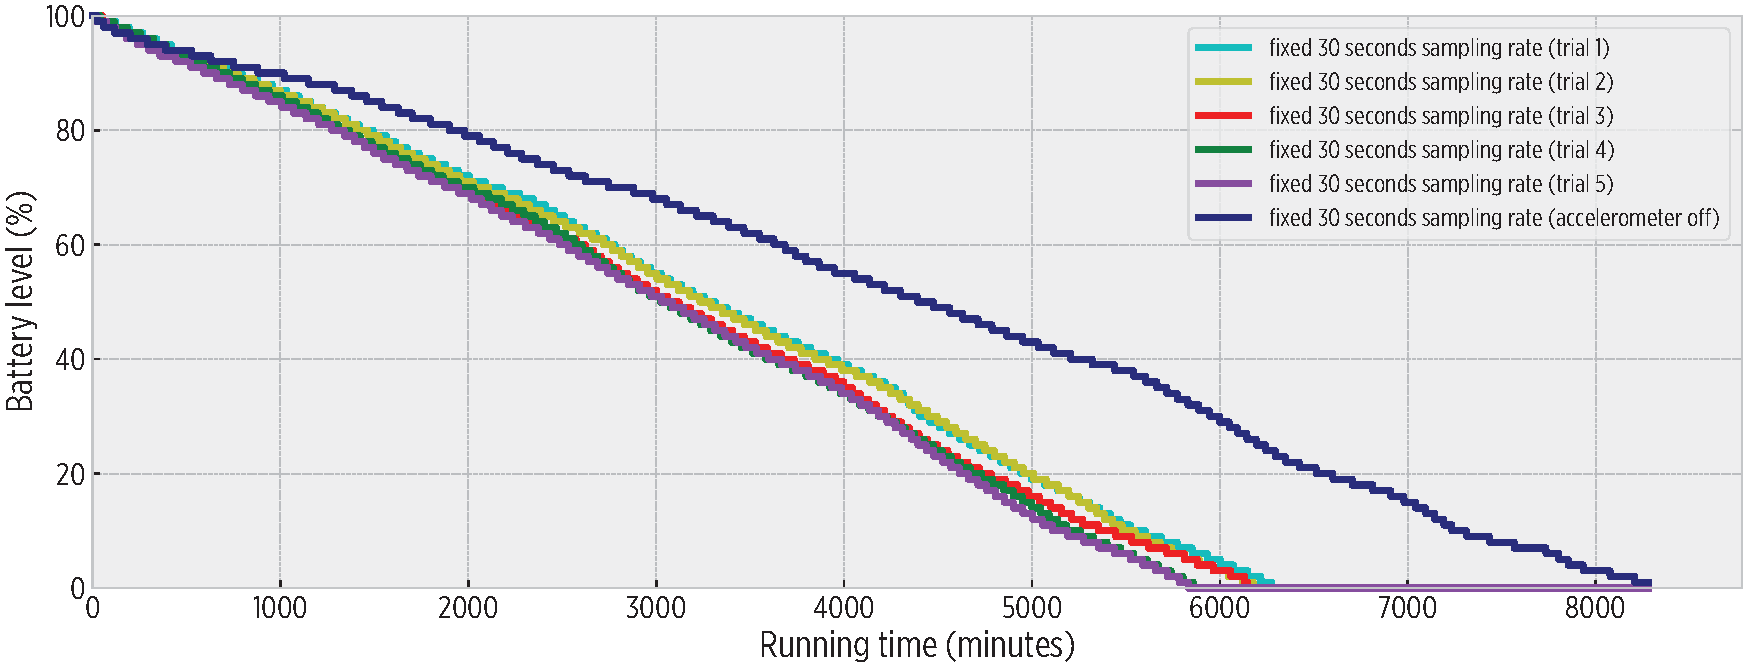
\includegraphics[width=0.8\textwidth]{vectors/experiments/preliminar-no-accelerometer}
  \caption{Energy consumption performance of the fixed 30 seconds GPS sampling trials with HAR module enabled, versus a fixed 30 seconds GPS sampling trial with HAR disabled. The battery lasts 1.5 days longer when HAR module is not enabled.}
\end{figure}
\end{frame}

\begin{frame}{Conclusions}{}
\small 
\begin{block}{\small \textbf{Conclusions}}
\begin{itemize}
  \item The experiments demonstrate the system's ability to identify the coarse-grain mobility events for building the STM. A first approximation shows that:% The first problem
  \begin{itemize}
  	\item Centroid distance between ground truth and observed stay points is at most $22.5 m$.
  	\item All stay points are detected, the arrival and departure latencies are within the active sampling rate.
  	\item The length of the visits missed by the \emph{Geofencing} are short, no longer than 4 minutes.
  \end{itemize}
  
  \item The STM information has proved its usefulness for the CC to reduce energy consumption with a minor impact on spatial-time accuracy: % The second problem

  \begin{itemize}
  	\item The latencies and spatial differences at arrival and departure events are within the expected values.
  	\item Only 33 – 49 \% of the location updates of a fixed $30 s$ sampling rate are employed in simulations.
  	\item On-device trials show a battery life increase of $26 - 76 h$, with respect of a fixed $30 s$ sampling rate.
  \end{itemize}

  \item The hypothesis is demonstrated as shown by the implementation of the CDS and the associated experimentation. %These results provide a solid evidence for demonstrating that the hypothesis implemented through the proposed CDS fulfills the objectives and contributions pursued by this research work.
  \item The EDS approach eases the design and implementation of the system, as it suits the characteristics of mobile platforms. Nevertheless, experimentation is needed to assess its energy performance.
  \item The developed middleware isolates sensors and power management complexity for long-term LBSs and MBSs.
  % \item The future work is mostly focused on final refinements of the solution and conducting experiments with a larger and heterogeneous mobility, as well as on its comparison against related solutions.
\end{itemize}
\end{block}

\end{frame}


\begin{frame}{Conclusions}{}
\small 
\begin{block}{\small \textbf{Doctoral program requirements}}
\begin{itemize}
  \item All the subject courses suggested by the admission committee were attended during the first year.
  \item A recommendation for refinement of the state of the art has been fulfilled.
  \item Such refinement and other advances performed on the research work has been submitted for publications (two journal articles \cite{Perez-Torres2016,Perez-Torres2016b}).
\end{itemize}
\end{block}

\end{frame}